% !TEX root = ../main.tex
\section{Vertikal integrasjon og market power}\label{thr:vertical-integration-market-power}

\paragraph{Definisjon.} Vertikal integrasjon kan brukes som et \emph{strategisk instrument} til å oppnå markedsmakt ved å kontrollere tilgang til essensielle inputs (oppstrøms) eller distribusjonskanaler (nedstrøms), og dermed stenge ute konkurrenter eller øke switching costs. BSZ kap.\ 19 presenterer modellen som viser hvordan en integrert produsent kan monopolisere nedstrømsmarkedet gjennom kontroll av et kritisk oppstrøms-input. [SLIDE]

\subsection*{Forklaring}

\textbf{Mekanismen.} Anta at en oppstrøms produsent $U$ er eneste kilde til et kritisk input. $U$ integrerer fremover (kjøper nedstrømsbedrift $D_1$). Nå kontrollerer $U$--$D_1$ tilgangen til input for rivaliserende nedstrømsaktører $D_2, D_3, \ldots$. $U$--$D_1$ kan: [SLIDE/BOK]

\begin{enumerate}\setlength{\itemsep}{2pt}
\item \textbf{Foreclosure:} Nekte å selge input til $D_2$, $D_3$ (eller sette prohibitiv pris) -- konkurrentene presses ut av markedet.
\item \textbf{Raising rivals' costs:} Selge input til $D_2$ til en høyere pris enn interne $D_1$ betaler -- $D_2$ taper kostnadskonkurranse.
\item \textbf{Kontroll av flaskehals:} Eierskap til infrastruktur (havn, rørledning, nett) gir gatekeeper-makt.
\end{enumerate}

\textbf{Resultat:} Nedstrømsmarkedet beveger seg mot monopol/duopol; sluttforbrukerpris stiger, kvantum synker, samfunnsmessig dødvektstap oppstår. Dette er et \emph{konkurranserettslig} problem -- regulering eller kartellmyndighet kan gripe inn (jf.\ \thref{market-failure-regulation}{regulering}). [BOK]

\subsection*{Grafisk modell -- vertikal integrasjon for market power}

\begin{figure}[h]
\centering
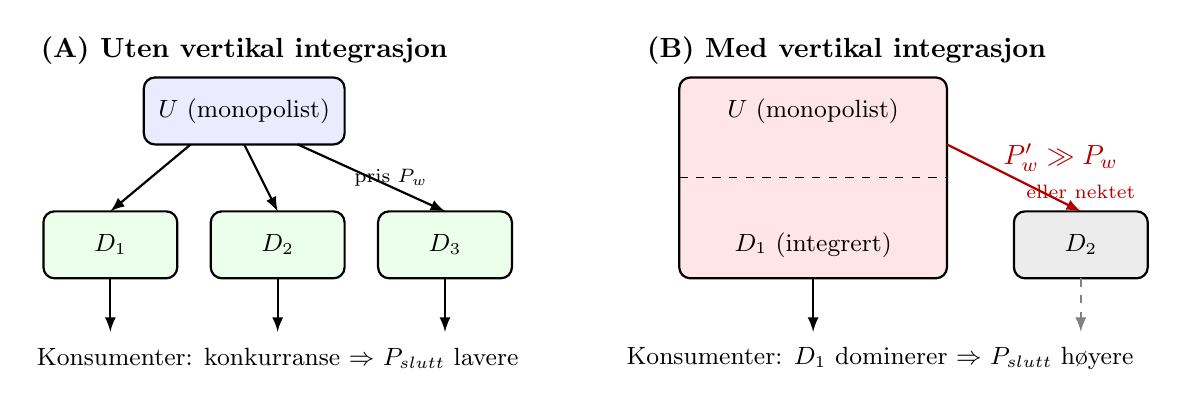
\begin{tikzpicture}[>=latex, scale=0.85, every node/.style={font=\small}]
  % --- Situasjon 1: Uten VI ---
  \node[font=\bfseries] at (3, 7.2) {(A) Uten vertikal integrasjon};
  % Upstream
  \draw[thick, rounded corners, fill=blue!8] (1.5,5.8) rectangle (4.5,6.8);
  \node at (3,6.3) {$U$ (monopolist)};
  % Downstream firms
  \draw[thick, rounded corners, fill=green!8] (0,3.8) rectangle (2,4.8);
  \node at (1,4.3) {$D_1$};
  \draw[thick, rounded corners, fill=green!8] (2.5,3.8) rectangle (4.5,4.8);
  \node at (3.5,4.3) {$D_2$};
  \draw[thick, rounded corners, fill=green!8] (5,3.8) rectangle (7,4.8);
  \node at (6,4.3) {$D_3$};
  % Arrows
  \draw[->, thick] (2.2,5.8) -- (1,4.8);
  \draw[->, thick] (3,5.8) -- (3.5,4.8);
  \draw[->, thick] (3.8,5.8) -- (6,4.8);
  \node[right] at (4.5,5.3) {\scriptsize pris $P_w$};
  % Konsumenter
  \draw[->, thick] (1,3.8) -- (1,3.0);
  \draw[->, thick] (3.5,3.8) -- (3.5,3.0);
  \draw[->, thick] (6,3.8) -- (6,3.0);
  \node at (3.5,2.6) {Konsumenter: konkurranse $\Rightarrow$ $P_{\text{slutt}}$ lavere};

  % --- Situasjon 2: Med VI ---
  \begin{scope}[xshift=9cm]
  \node[font=\bfseries] at (3, 7.2) {(B) Med vertikal integrasjon};
  % Integrert firma
  \draw[thick, rounded corners, fill=red!10] (0.5,3.8) rectangle (4.5,6.8);
  \node at (2.5,6.3) {$U$ (monopolist)};
  \node at (2.5,4.3) {$D_1$ (integrert)};
  \draw[dashed] (0.5,5.3) -- (4.5,5.3);
  % Rivaler
  \draw[thick, rounded corners, fill=gray!15] (5.5,3.8) rectangle (7.5,4.8);
  \node at (6.5,4.3) {$D_2$};
  % Arrow med X
  \draw[->, thick, red!70!black] (4.5,5.8) -- (6.5,4.8);
  \node[red!70!black, font=\bfseries] at (6.2,5.6) {$P_w' \gg P_w$};
  \node[red!70!black, font=\scriptsize] at (6.5,5.1) {eller nektet};
  % Konsumenter
  \draw[->, thick] (2.5,3.8) -- (2.5,3.0);
  \draw[->, thick, dashed, gray] (6.5,3.8) -- (6.5,3.0);
  \node at (3.5,2.6) {Konsumenter: $D_1$ dominerer $\Rightarrow$ $P_{\text{slutt}}$ høyere};
  \end{scope}
\end{tikzpicture}
\caption{\textbf{Vertikal integrasjon for market power.} (A) Uten VI: oppstrøms monopolist $U$ selger til alle nedstrøms-aktører til pris $P_w$; konkurranse blant $D_1$--$D_3$ holder sluttprisen nede. (B) Med VI: $U$--$D_1$ integrert; rivalen $D_2$ nektes input eller betaler prohibitiv pris $P_w'\gg P_w$ (\emph{foreclosure / raising rivals' costs}). $D_1$ får markedsmakt nedstrøms, sluttprisen stiger. [SLIDE/BOK -- BSZ kap.\ 19]}
\end{figure}

\subsection*{Kjerneforutsetninger}
\begin{itemize}
\item Oppstrøms monopol (eller sterk markedsposisjon) -- uten dette kan ikke foreclosure fungere.
\item Nedstrømsmarkedet er imperfekt: rivaler kan ikke skaffe input fra andre kilder.
\item Ingen effektiv regulering som forbyr foreclosure.
\item Integrert firma har incentiv til å begrense konkurranse (profitt fra monopolisering > tap fra redusert upstream-salg til rivaler).
\end{itemize}

\subsection*{Muligheter}
\begin{itemize}
\item Forklarer hvorfor konkurransemyndigheter (EU DG Comp, US DOJ) gjennomgår vertikale fusjoner.
\item Predikerer i hvilke industrier VI gir markedsmakt: flaskehals-industrier (nettverk, infrastruktur, sjeldne råvarer).
\item Gir normativt grunnlag for regulering av nettnøytralitet, tilgang til infrastruktur og essensiell fasilitets-doktrine.
\end{itemize}

\subsection*{Begrensninger og kritikk}
\begin{itemize}
\item Chicago School-kritikken: VI skaper ikke ny monopolmakt -- oppstrømsmonopolisten kan allerede ekstrahere all monopolprofitt via inputpris. VI er da nøytral eller effektivitetsfremmende (eliminerer double markup).
\item Forutsetter at oppstrøms monopol er varig -- entry, innovasjon eller substitutter kan undergrave foreclosure.
\item Reguleringsmyndigheter kan pålegge tilgangsforpliktelser (unbundling, FRAND-lisenser) som gjør foreclosure umulig.
\item Modellen er statisk; dynamisk kan rivaler tilpasse seg (bakoverintegrasjon, finne alternativt input).
\end{itemize}

\subsection*{Eksempler}
\begin{itemize}\setlength{\itemsep}{2pt}
\item \textbf{De Beers og diamantdistribusjon.} De Beers kontrollerte oppstrøms gruvedrift og brukte integrert distribusjon (Central Selling Organisation) til å kontrollere globale diamantpriser i tiår. Foreclosure av uavhengige slipere/forhandlere var nøkkelen. [EKS]
\item \textbf{Google/Alphabet og Android.} EU-kommisjonen bøtelagte Google (2018) for å bruke Android (oppstrøms OS) til å tvinge forinstallering av Google-apper (nedstrøms tjenester) -- klassisk leveraging av oppstrøms dominans til nedstrøms foreclosure. [EKS]
\item \textbf{Standard Oil (1870--1911).} Rockefeller integrerte bakover i rørledninger og fremover i distribusjon for å stenge ute rivaler. US Supreme Court påla oppløsning i 1911. [EKS]
\end{itemize}

\subsection*{Kobling til søyle og andre teorier}
Søyle: \SOne\ (eierskap som kontrollrett over verdikjede). Relaterte: \thref{vertical-integration-outsourcing}{Vertikal integrasjon og outsourcing}, \thref{boundaries-of-the-firm}{Boundaries of the Firm}, \thref{double-markup-problem}{Double markup} (Chicago-motargumentet), \thref{market-failure-regulation}{Regulering} (myndighetenes respons), \thref{externalities}{Eksternaliteter} (markedsmakt skaper negativ eksternalitet for konsumenter).

\paragraph{Brukt i spørsmål:} Q11.
